\chapter{Projectgrenzen}
In dit hoofdstuk worden de projectgrenzen toegelicht.
De afbakening van het project ligt toe wat er wel en niet gemaakt binnen de context van de afstudeer opdract.
Vervolgens wordt de definition of done beschreven om aan te tonen wanneer de opdracht voldaan is.
Daarna worden de randvoorwaarden van de afstudeeropdracht besproken.
\section{Afbakening}
De opdracht wordt beperkt tot het ontwerpen en ontwikkelen van de \gls{CMS}-API en een interface applicatie om de content van de \gls{CMS}-API te tonen.
Er is besloten om geen \gls{GUI} te maken voor de klanten op de \gls{CMS}-API om de scope en lengte van het project haalbaar te maken.
In figuur \ref{fig:ProductOverview} is te zien welke onderdelen gemaakt worden.
Om toch de user journeys kunnen valideren wordt dit getest door middel van postman workflows.
Er wordt wel een frontend applicatie gemaakt voor het renderen van de content, deze applicatie zal wel minimaal blijven.
\begin{graphic}
    \captionsetup{type=figure}
    \caption{producten die gemaakt worden tijdens de afstudeeropdracht}
    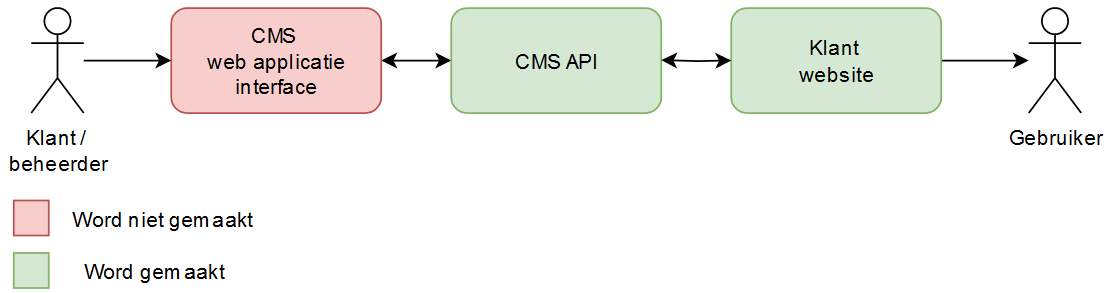
\includegraphics[scale=0.4]{ProductOverview}
    \label{fig:ProductOverview}
\end{graphic}
\whitespace
\textbf{Wel:}
\whitespace
- minimaal uitwerken van de \qw{must haves vanuit} de aanbevelingen van het onderzoek.
\todo[inline]{gevoel dat hier nog extra dingen bij moeten staan.}
\textbf{Niet:}
\whitespace
- een \gls{CMS} interface maken waarmee de klant content kan plaatsen voor de gebruiken.\\
- de won't haves die van uit de aanbevelingen van het onderzoek komen uitwerken.
\section{Definition of done}
De definition of done is wanneer er een proof of concept CMS-API en de daarbij behorende frontend is opgeleverd. 
Die voldoen aan de eisen en wensen die uit het ondezoek zijn gekomen van de stakeholders.
Het systeem moet flexibel opgesteld worden, zodat in de toekomst extra functionaliteiten toegevoegd kunnen worden.
\todo[inline]{meer?} 
Daarnaast is het van belang dat de school documentatie met een voldoende wordt afgerond.
De verschillende documenten zijn: plan van aanpak, onderzoek, technisch verslag.
Daarna moet het product en de presentatie met een voldoende afgerond worden.
\section{Randvoorwaarden}
Om het project goed af te kunnen ronden zijn er randvoorwaarden aan het project verbonden: \\
- Er is een werk plek nodig om alle werkzaamheden tijdens de afstudeerperiode te kunnen afronden.\\
- Er moet voldoende contact gehouden worden met de bedrijfsbegeleider en de docentbegeleider. \\ 
- de afstudeerperiode duur is ongeveer 125 werkdagen en loopt van 6 oktober 2023 tot 5 april 2024.
